\documentclass[10pt]{standalone}
\usepackage{amsmath}
\usepackage{amssymb}
\usepackage{pgf,tikz}
\usepackage{mathrsfs}
\usetikzlibrary{arrows}
\pagestyle{empty}

\begin{document}

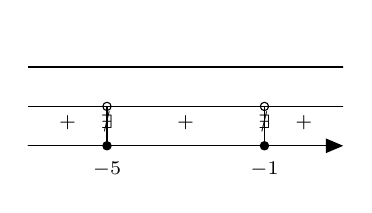
\begin{tikzpicture}[line cap=round,line join=round,>=triangle 45,x=1.0cm,y=1.0cm]

\draw[->] (0.,0.) -- (4.,0.);


\clip(0.,-0.5) rectangle (4.,1.5);
\draw (0.,0.5)-- (4.,0.5);
\draw (1.,0.5)-- (1.,0.);
\draw (3.,0.5)-- (3.,0.);
\draw (0.,1.)-- (4.,1.);
\begin{scriptsize}
\draw [fill=black] (1.,0.) circle (1.5pt);
\draw[color=black] (1.0,-0.3) node {$-5$};
\draw [fill=black] (3.,0.) circle (1.5pt);
\draw[color=black] (3.0,-0.3) node {$-1$};
\draw  (1.,0.5) circle (1.5pt);
\draw  (3.,0.5) circle (1.5pt);
\draw[color=black] (3.0,0.3) node {$\nexists$};
\draw[color=black] (1.0,0.3) node {$\nexists$};
\draw[color=black] (0.5,0.3) node {$+$};
\draw[color=black] (2.0,0.3) node {$+$};
\draw[color=black] (3.5,0.3) node {$+$};

\end{scriptsize}
\end{tikzpicture}
\end{document}